\section{Related Work}

Recent advancements in cloud computing, WebAssembly, and energy-efficient frameworks have sparked numerous innovations in system design and optimization. This section reviews notable contributions in WebAssembly enhancements, energy optimization in large-scale training and inference systems. These works highlight the state-of-the-art methodologies and provide a foundation for our proposed approach.

% \subsection{Function as a Function}

% Function as a Function \cite{kuchler2023function} propose dandelion, a FaaS system that adds a new programming paradigm where functions are divided into compute and IO functions. Developers create the compute functions and agglomerate them with IO functions into what they call compositions. This programming model makes it easier to achieve isolation and thus runtimes do not need to be recreated like in the Firecracker micro VM. This achieves 45x lower tail latency (latency of the highest latency requests) for cold starts.

% As with the microservice frameworks Service Weaver and Blueprint, this work is not seamless and is dependent on a new framework.

% With the arrival of WebAssembly however, since it already provides a trusted system interface (WASI), there’s no need for this programming model of separating IO and compute.

\subsection{Bringing WebAssembly Up to Speed with Dynamic Linking}
\label{sec-3.1}

Recent advances in WebAssembly (Wasm) have expanded its applicability beyond web applications to include cloud computing, edge devices, and distributed systems. However, its lack of built-in support for dynamic linking presents significant challenges when designing modular and efficient distributed applications. Addressing this gap, the work by Makitalo et al. \cite{makitalo2021bringing} develops a custom runtime based on WasmTime that extends its capabilities to implement dynamic linking.

In their approach, they parse the dylink.0 custom section of shared library WebAssembly modules.
This section encodes metadata, including:

\begin{itemize}
\item Shared library dependencies,
\item Memory size and alignment requirements,
\item Function table requirements.
\end{itemize}

Using this metadata, the authors implement the \textit{\textbf{dlopen}} and \textit{\textbf{dlsym}} functions, which are not natively supported in WASI v1. These functions enable runtime linking of shared libraries.

We build upon this work as the basis for our initial solution proposal to enable remote module execution.


% \begin{figure}[h!]
% \centering
% 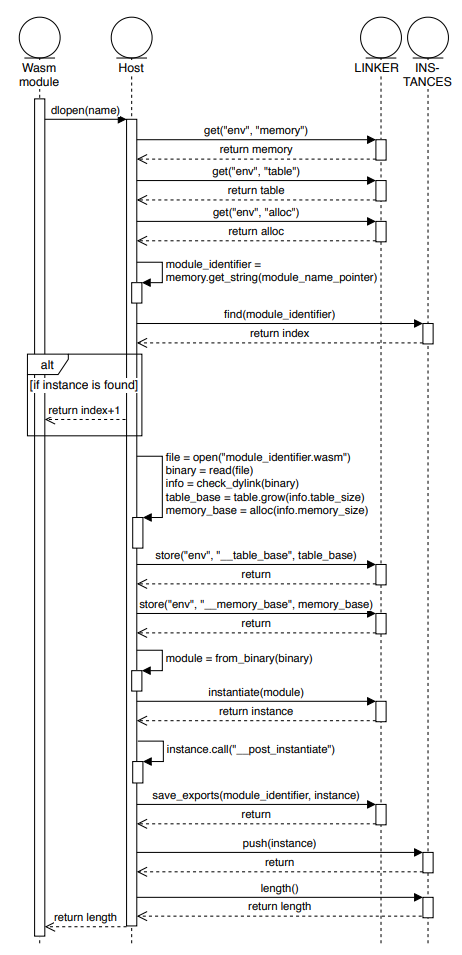
\includegraphics[width=0.5\textwidth]{Images/dynamic-linking-flow.png}
% \caption{Sequence diagram of the \textit{\textbf{dlopen}} function call by Makitalo et al. \cite{makitalo2021bringing}}
% \label{fig:dynamic-linking-flow}
% \end{figure}

\subsection {Reducing Energy Bloat in Large Model Training
}

Training large AI models on numerous GPUs consumes a massive amount of energy, making power delivery one of the largest limiting factors in building and operating datacenters for AI workloads. However, as demonstrated by the work on Perseus \cite{chung2024reducing}, not all energy consumed during training directly contributes to end-to-end throughput. A significant portion can be removed without slowing down training. This portion is referred to as energy bloat.

The work on Perseus addresses this issue by identifying two independent sources of energy bloat in large model training and proposing a training system to mitigate both by slowing down the frequencies of the individual Streaming MultiProcessors in Nvidia GPUs.

One possible cost optimization we could include in our work would be to downsize the hardware when the frequency achieves a certain threshold, but it is not clear whether this would bring any benefit due to the high-bandwidth mesh that is used for these clusters. This work is also focused on training as opposed to our work on inference.

\subsection {DynamoLLM: Designing LLM Inference Clusters
for Performance and Energy Efficiency}

The paper introduces DynamoLLM\cite{dynamollm}, an energy-management framework for Large Language Model (LLM) inference clusters. DynamoLLM\cite{dynamollm} aims to optimize the energy efficiency and cost of LLM serving while meeting Service Level Objectives (SLOs) such as latency constraints, to do this they exploit the \textbf{heterogeneity} and \textbf{fluctuations} in the inference workloads.

This \textbf{heterogeneity} can be found in the computational phases of LLMs, where first, in the prefill phase, input tokens are computed in parallel, and, in the second phase, the decode phase, the LLM autoregressively generates the output tokens. Since the number of output tokens is not known at request time, they predict this number. One example of an optimization they do is that they then use the input and output token length and select the appropriate pool with the correct model parallelism and gpu frequency configuration based on energy consumption historical data. One example of a energy consumption profile for a Llama2-70B can be seen in Figure \ref{fig:dynamo-llm}.

\begin{figure}[h!]
\centering
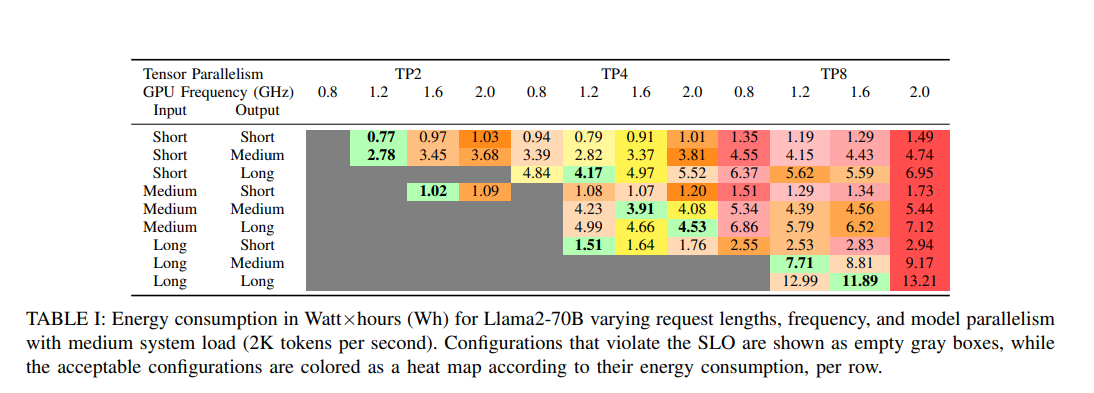
\includegraphics[width=1.0\textwidth]{Images/dynamo-llm.png}
\caption{Dynamo-LLM\cite{dynamollm} Energy Consumption with varying input and output tokens.}
\label{fig:dynamo-llm}
\end{figure}

\subsubsection*{DynamoLLM Framework}
Some of the key features of this framework include:
\begin{enumerate}
    \item \textbf{Instance Reconfiguration:} Dynamically adjusts the number of instances, GPU frequency, and model parallelism.
    \item \textbf{Hierarchical Controllers:} Divides control tasks across cluster, pool, and instance levels.
    \item \textbf{Predictive Scheduling:} Predicts request types, such as output token length and adjusts resource allocation accordingly.
\end{enumerate}

\subsubsection*{Evaluation}

The framework was evaluated on a large-scale GPU cluster using production-level workloads with the following results:

\begin{itemize}
    \item \textbf{Energy Savings:} DynamoLLM conserves 53\% energy compared to traditional setups.
    \item \textbf{Carbon Emission Reduction:} Achieves a 38\% reduction in operational carbon emissions.
    \item \textbf{Cost Efficiency:} Reduces operational costs by 61\% while meeting latency requirements (SLOs)
\end{itemize}

One possible downside this work might have is possibly having fixed hardware type for the pools, since the code is not provided, there's no guarantee, but based on the evaluation they've done (only H100's), it might not support true downscaling to cheaper GPU's and possibly CPU VM's with vertical scaling as our work does.

\subsection{Discussion}

The reviewed works address specific challenges in their respective domains, but gaps remain that our proposal targets.

The work by Makitalo et al. extends WebAssembly with dynamic linking, enabling runtime library loading via \textit{dlopen} and \textit{dlsym}, and we use its ideas for our initial remote module execution proposal.

Perseus optimizes GPU frequency management to reduce energy consumption during large-scale model training. Although effective for training, it does not address inference-specific requirements. Our work extends dynamic resource allocation to heterogeneous hardware, focusing on inference workloads and enabling cost-efficient scaling.

DynamoLLM improves energy efficiency and performance for LLM inference clusters through workload-specific optimizations. However, its design seems to not allow vertical scaling, only horizontal scaling via adding more instances, this limits its applicability to lower-cost hardware configurations. Our proposal supports both vertical and horizontal scaling and integrates WebAssembly for extensibility and portable execution across cloud and edge environments.